%%%%%%%%%%%%%%%%%%%%%%%%%%%%%%%%%%%%%%%%%
% Short Sectioned Assignment
% LaTeX Template
% Version 1.0 (5/5/12)
%
% This template has been downloaded from:
% http://www.LaTeXTemplates.com
%
% Original author:
% Frits Wenneker (http://www.howtotex.com)
%
% License:
% CC BY-NC-SA 3.0 (http://creativecommons.org/licenses/by-nc-sa/3.0/)
%
%%%%%%%%%%%%%%%%%%%%%%%%%%%%%%%%%%%%%%%%%

%----------------------------------------------------------------------------------------
%	PACKAGES AND OTHER DOCUMENT CONFIGURATIONS
%----------------------------------------------------------------------------------------

\documentclass[paper=a4, fontsize=11pt]{scrartcl} % A4 paper and 11pt font size

\usepackage[pdftex]{graphicx}  
\usepackage{subfig}   

\usepackage[T1]{fontenc} % Use 8-bit encoding that has 256 glyphs
\usepackage{fourier} % Use the Adobe Utopia font for the document - comment this line to return to the LaTeX default
\usepackage[english]{babel} % English language/hyphenation
\usepackage{amsmath,amsfonts,amsthm} % Math packages

\usepackage{xcolor}
\usepackage{listings}

\usepackage{url}

\usepackage{sectsty} % Allows customizing section commands
\allsectionsfont{\centering \normalfont\scshape} % Make all sections centered, the default font and small caps

\usepackage{fancyhdr} % Custom headers and footers
\pagestyle{fancyplain} % Makes all pages in the document conform to the custom headers and footers
\fancyhead{} % No page header - if you want one, create it in the same way as the footers below
\fancyfoot[L]{} % Empty left footer
\fancyfoot[C]{} % Empty center footer
\fancyfoot[R]{\thepage} % Page numbering for right footer
\renewcommand{\headrulewidth}{0pt} % Remove header underlines
\renewcommand{\footrulewidth}{0pt} % Remove footer underlines
\setlength{\headheight}{13.6pt} % Customize the height of the header

\numberwithin{equation}{section} % Number equations within sections (i.e. 1.1, 1.2, 2.1, 2.2 instead of 1, 2, 3, 4)
\numberwithin{figure}{section} % Number figures within sections (i.e. 1.1, 1.2, 2.1, 2.2 instead of 1, 2, 3, 4)
\numberwithin{table}{section} % Number tables within sections (i.e. 1.1, 1.2, 2.1, 2.2 instead of 1, 2, 3, 4)

\setlength\parindent{0pt} % Removes all indentation from paragraphs - comment this line for an assignment with lots of text

%----------------------------------------------------------------------------------------
%	TITLE SECTION
%----------------------------------------------------------------------------------------

\newcommand{\horrule}[1]{\rule{\linewidth}{#1}} % Create horizontal rule command with 1 argument of height

\title{	
\normalfont \normalsize 
\textsc{UGR, ETSIIT} \\ [25pt] % Your university, school and/or department name(s)
\horrule{0.5pt} \\[0.4cm] % Thin top horizontal rule
\huge Developement of a power grid ontology and a sample application \\ % The assignment title
\horrule{2pt} \\[0.5cm] % Thick bottom horizontal rule
}

\author{Felipe Oehrwald, Clemens von Schwerin}
\date{\normalsize\today} % Today's date or a custom date

\begin{document}

\maketitle % Print the title

\section{Introduction}

The Semantic Web extends the Web to make data between computers easier to exchange and easier to use. The term "Granada"
can be supplemented, for example, in a web document with the information as to whether a ship name, family name or town
name is meant here. This additional information explicates the otherwise unstructured data. Standards are used for the
publication and use of machine-readable data. While people can close such information from the given context and
unconsciously build such links, machines must first be brought to this context. For this purpose, the content is linked
with further information and Web Ontology Language (OWL) is a way to write domains and their relationships formally. OWL
is a specification of the World Wide Web Consortium (W3C) to create, publish and distribute ontologies using a formal
description language.\\

This paper therefore creates a an power grid ontology as a general use case in Section II. Section III delineates the general challenge arising with the regard to the integration of Java Application to OWL Ontologies and presents existing technical approaches. Section IV provides an outlook and discusses the suitability for use cases with focus on integration and multi-platform approaches.
\newpage

\section{Ontology details}

The power grid ontology is aimed to give a basis for representing power grids in terms of power production, consumption and transmission. For that purpose the following classes, as listed in figure \ref{fig:classes} were designed.
The most basic building blocks are the \textit{NetworkEntities} which model all physical entities 
a network may consist of and are disjoint. There are \textit{Producers} adding power to the network, \textit{Consumers} drawing energy from the network, \textit{TransportEntities} transporting the energy between exactly two other network entities and \textit{Transformers} managing splits, merges and changes in the transmission type of \textit{TransportEntities}. \\
Those transmission types are modelled in the \textit{TransmissionType} class. This class is divided into two disjoint subclasses \textit{ACTransmission} for alternating current and \textit{DCTransmission} for direct current. \\
Each \textit{TransportEntity} furthermore has a \textit{CableType} indicating the layout of a power line. There are 3 disjoint alternatives: regular \textit{TransmissionLines}, \textit{UndergroundCables} and \textit{UnderseaCables}. \\
Finally every \textit{NetworkEntity} is part of a specific \textit{Network}.

\begin{figure}
\centering
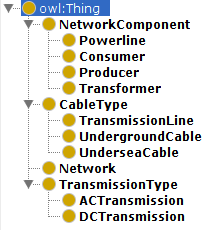
\includegraphics[scale=.75]{img/classes.png} 
\label{fig:classes}
\caption{Class hierarchy of the Power Grid ontology.}
\end{figure}

\section{Processing OWL Ontologies using Java}

In the following, Java code will be presented to make requests on the build ontology in section II. For this task we the \textit{OWL API}. The \textit{OWL API} is a \textit{Java API} and reference implmentation for creating, manipulating and serialising \textit{OWL Ontologies}. The latest version of the API is focused towards \textit{OWL 2}. The challenges that are to be addressed can be illustrated with a simple scenario. We assume that an energy provider is trying to receive information over his power grid on a dashboard that is written in Java Code. In the \textit{OWL API}, an \textit{OWLOntology} is an interface, modeling a set logical and non-logical \textit{OWLAxioms}, with a name (an IRI), a physical location and convenience methods to retrieve such axioms. An \textit{IRI} allows easily identifying \textit{OWLEntities}. Furthermore, class names, data, object properties, annotation properties and named individuals.\\

First of all, we create two variables to load an ontology from an existing file. There are different ways to read and work with \textit{OWL Files}. One option is to work with the \textit{OWLOntologyManager}. \textit{OWLOntologies} are created by \textit{OWLOntologyManager} and all other interfaces are built using \textit{OWLDataFactory}. 

\begin{figure}[h]
\centering
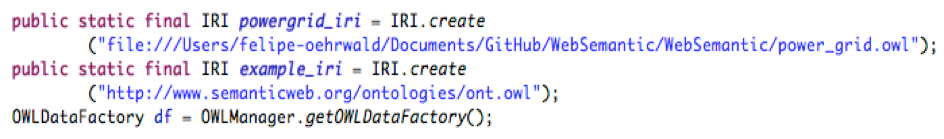
\includegraphics[width=\textwidth]{img/load.png}
\caption{Load an IRI based on the OWL File.}
\label{fig:Load}
\end{figure}

\begin{figure}[h]
\centering
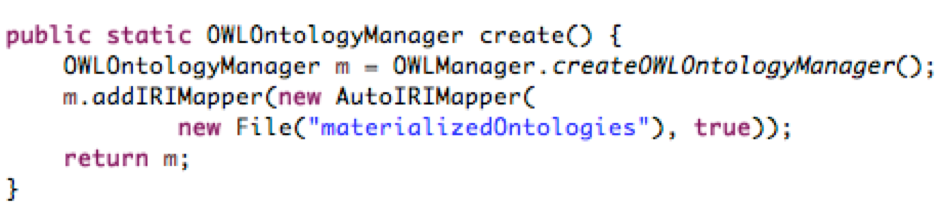
\includegraphics[width=\textwidth]{img/create.png}
\caption{Creates an IRI based on the OWL File.}
\label{fig:Create}
\end{figure}

\newpage

\begin{figure}[h]
\centering
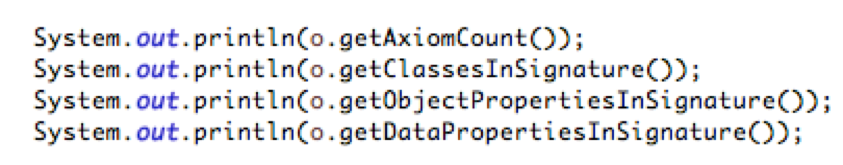
\includegraphics[width=\textwidth]{img/apiCall.png}
\caption{Executing request on OWL Ontology.}
\label{fig:apiCall}
\end{figure}

\begin{figure}[h]
\centering
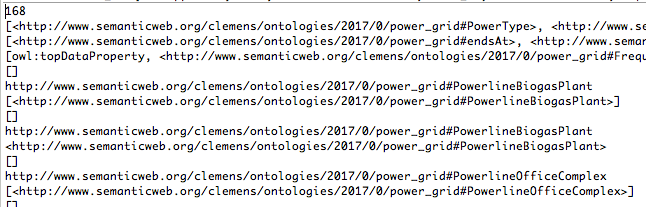
\includegraphics[width=\textwidth]{img/request.png}
\caption{Result of the Java Request.}
\label{fig:request}
\end{figure}

\\
The output reveals that it is possible to run simple request on an OWL Ontology that have been created in Protege. 
With the request we received the size  of the classes that are in the signature of this object (168 in total) or the names of the classes that have been build in the referenced ontology.

\newpage

 



\section{Outlook}

In this paper, we highlighted the enormous impact of web ontologies itself and the capabilities of web ontologies in combination with Java Application. We analyzed several existing approaches for technically supporting such integration. From the perspective of integration as well as from a broader view of a modest installation web ontologies fail to keep promise of an overall flexible environment in style of MEAN stack software bundle. Although, it shares the same implementation steps as relational database services (MySQL) in Java Application the effort is pretty high to connect OWL to Java Application. Moreover, the amount available use cases and best practice approaches is still limited. This is due to the fact, that Web Semantic is as yet less popular inside the communities and this therefore needs to be further incentivized to raise popularity. A possibility can be the use of D2R Server. D2R Server allow to publish the content of relational databases on the Semantic Web in which it maps databases into RDF format.\\ 

There is thus a clear need for developing appropriate mechanisms to connect Java Application to OWL Files andto unleash the full potential of web ontologies. For further research, it would be interesting to work with Python, as a programming language with less leverage. Furthermore, it would be intressting to do a benchmarking between Java and Python in regard to OWL Files. Nevertheless,  Web Ontologies will become more and more important. With the emerge of Open Data Government policies, that allow free access to machine readable information, web semantic technologies like for instance RDF will play an important role in the future in scraping and linking data.

\newpage

\bibliographystyle{plain}
\bibliography{documentation}

\end{document}